

\section* {Supplemental information}

\beginsupplement



\section*{Supplemental Figures}

\begin{figure*}[!hbtp]
    \centering
    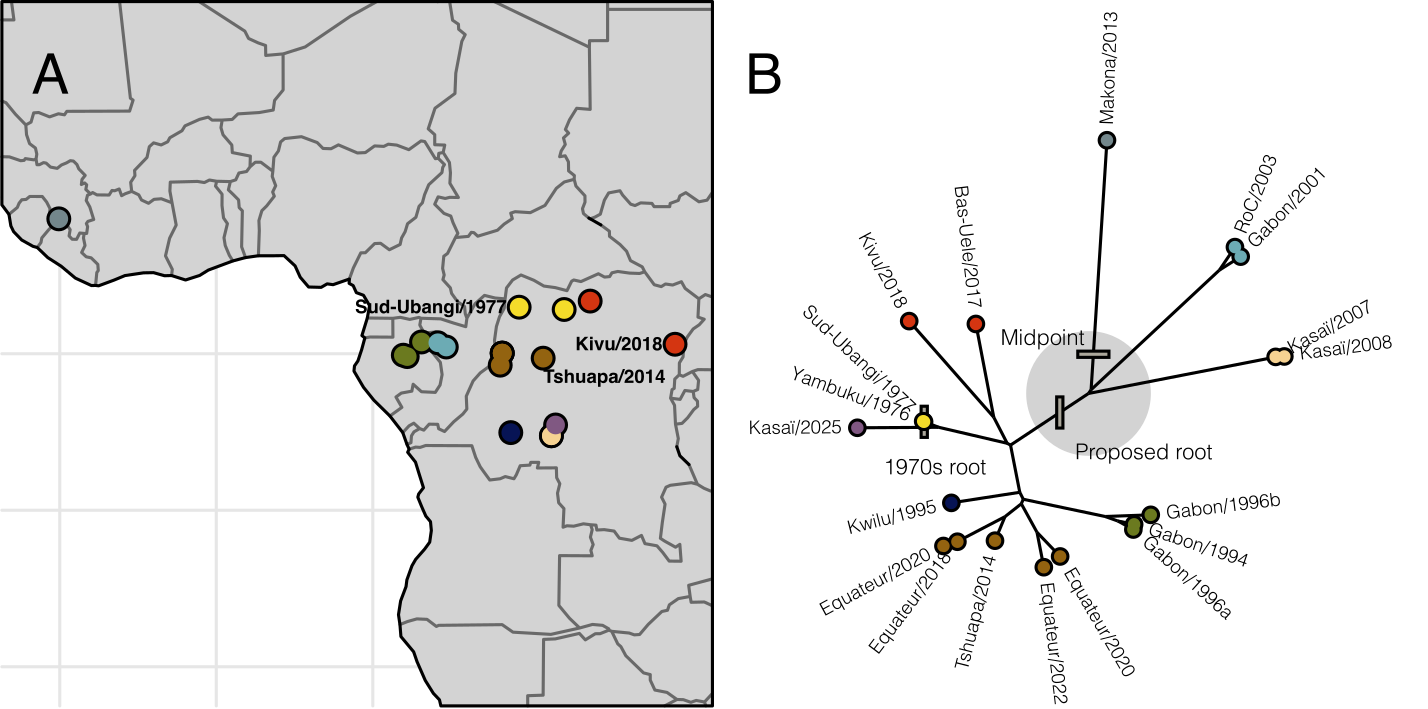
\includegraphics[width=1\textwidth]{figures/mapFigure.png}
    \caption{\textbf{A map (A) and unrooted tree (B) representing the outbreaks included in this study.} Common and proposed root placements are noted on the tree. The large grey sphere represents plausible root positions proposed by the latency rate model.}
    \label{fig:map}
\end{figure*}

\begin{figure*}[!hbtp]
    \centering
        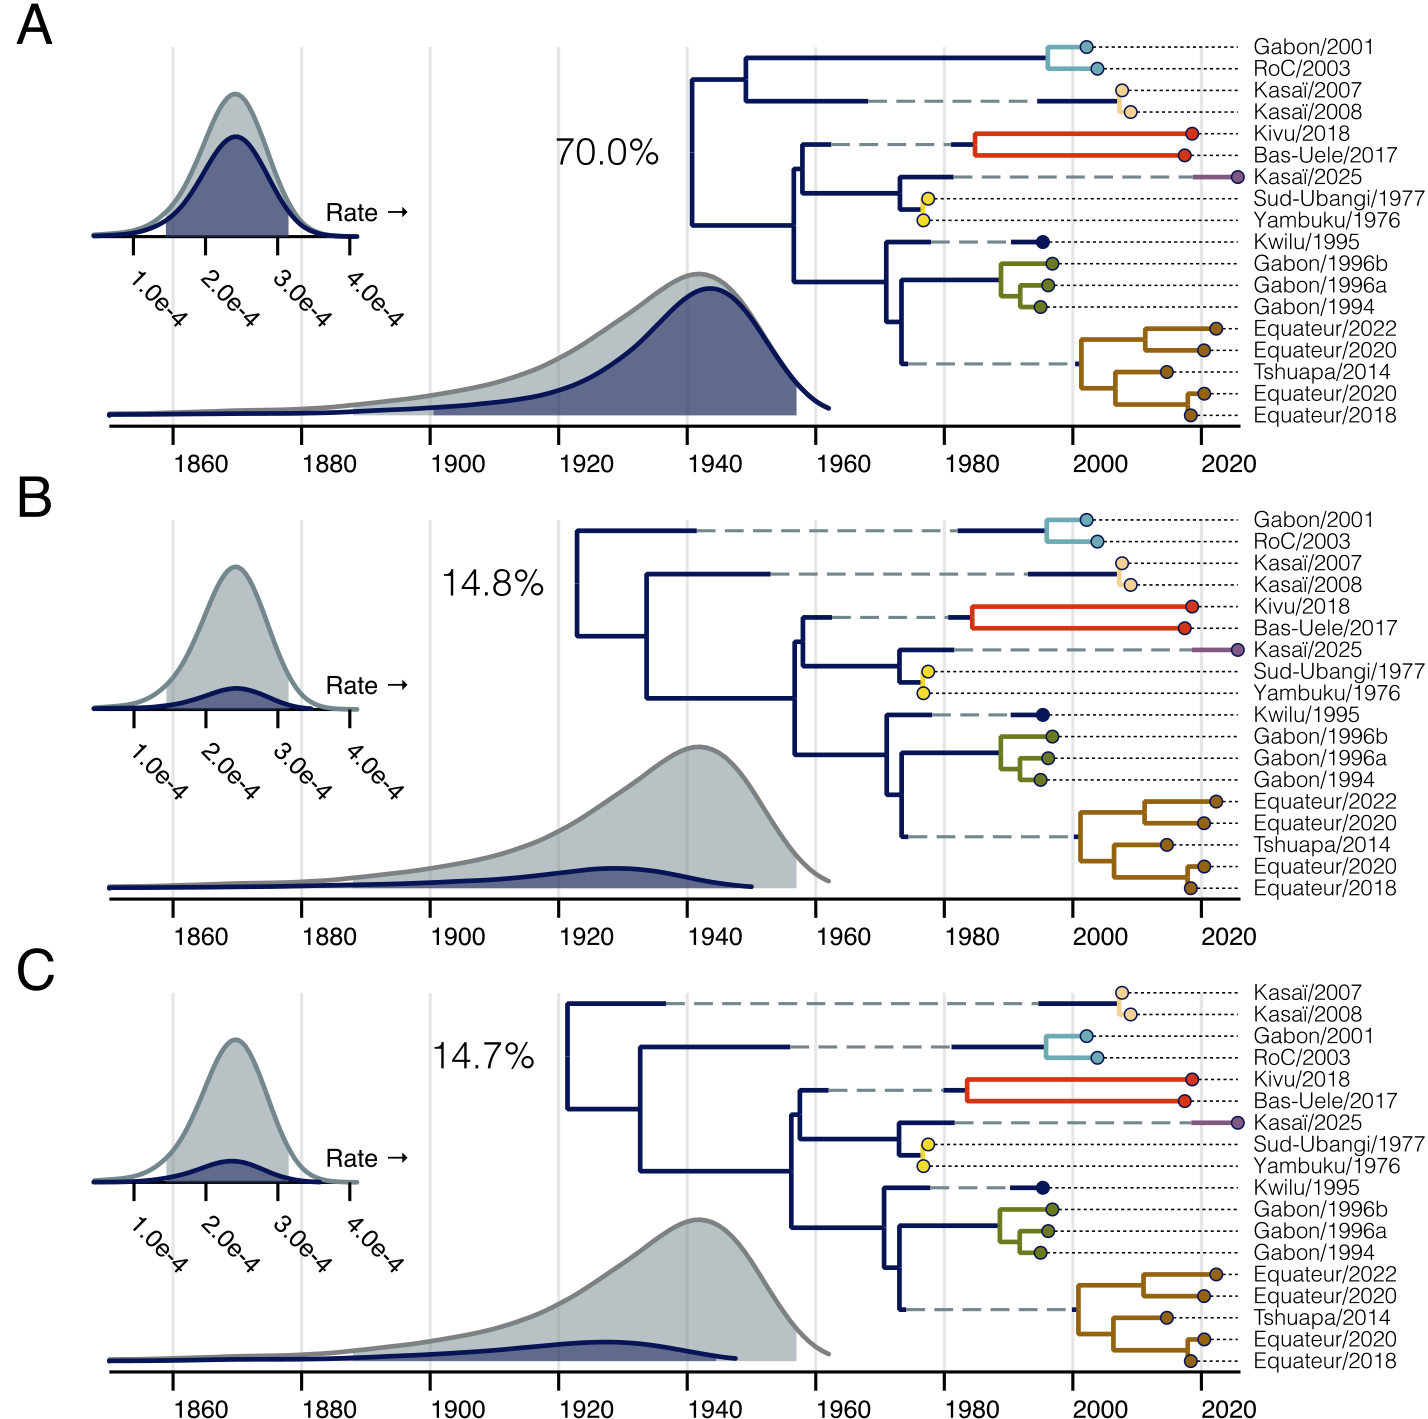
\includegraphics[width=1\textwidth]{figures/allRoots.noMakona.png}
   \caption{
     \textbf{The evolutionary history of EBOV in Central Africa under the latent model (all explored roots).} 
	Same as Figure~\ref{fig:scNmBEAST} but for all rootings with greater than 5\% posterior support.
   } 
    \label{fig:nMallRoots}
\end{figure*}

\begin{figure*}[!hbtp]
    \centering
        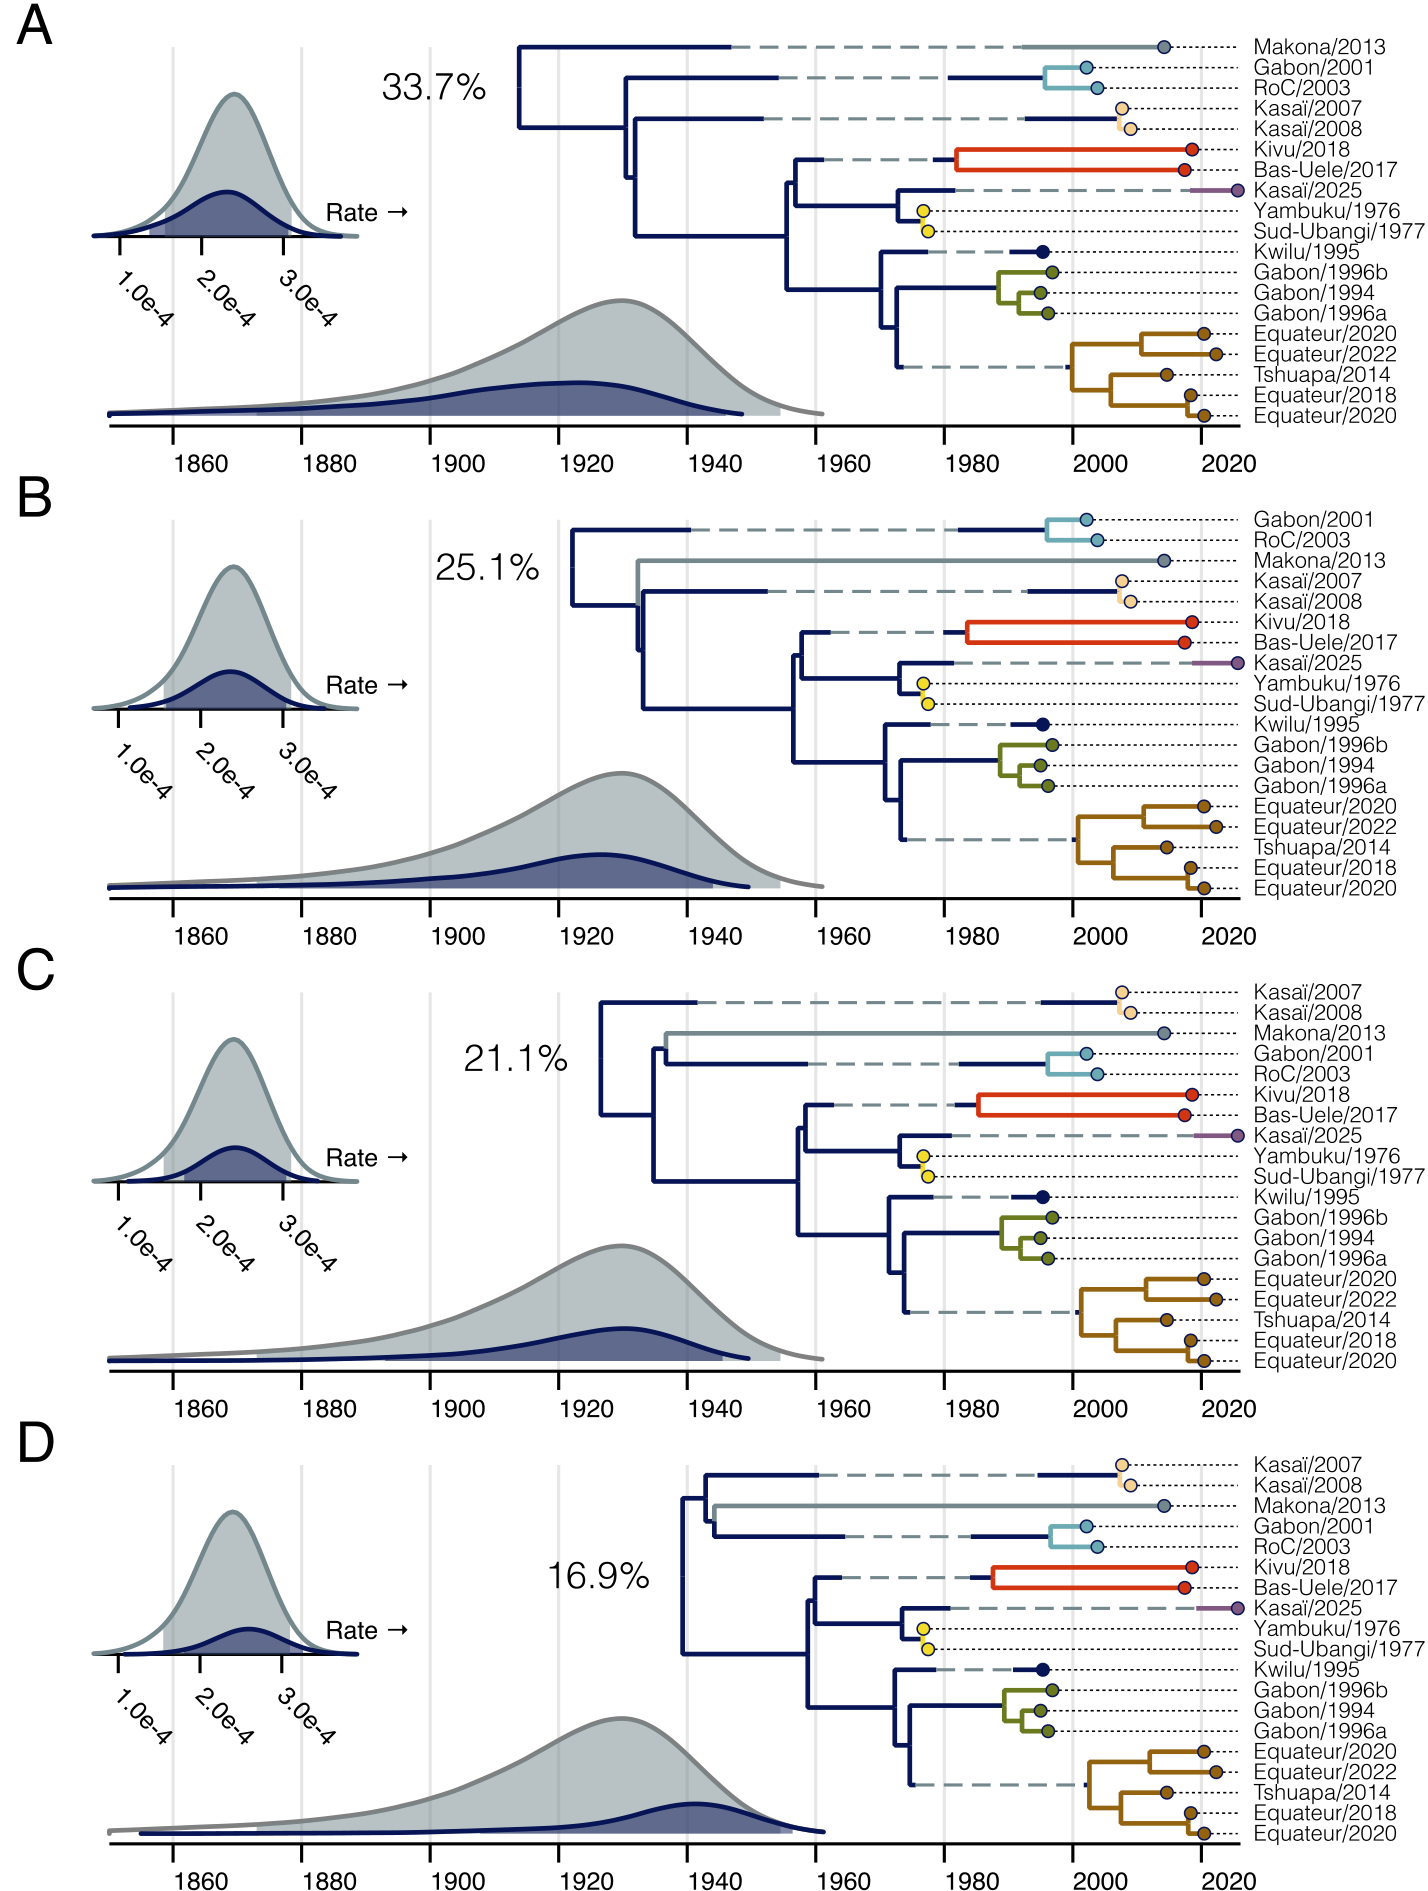
\includegraphics[width=1\textwidth]{figures/allRoots.png}
    \caption{\textbf{The evolutionary history of all EBOV outbreaks under the latent model partitioned by root position (all explored roots).} 
	Same as Figure~\ref{fig:scBEAST} but for all rootings with greater than 5\% posterior support.
   } 
    \label{fig:allRoots}
\end{figure*}

\begin{figure*}[!hbtp]
    \centering
    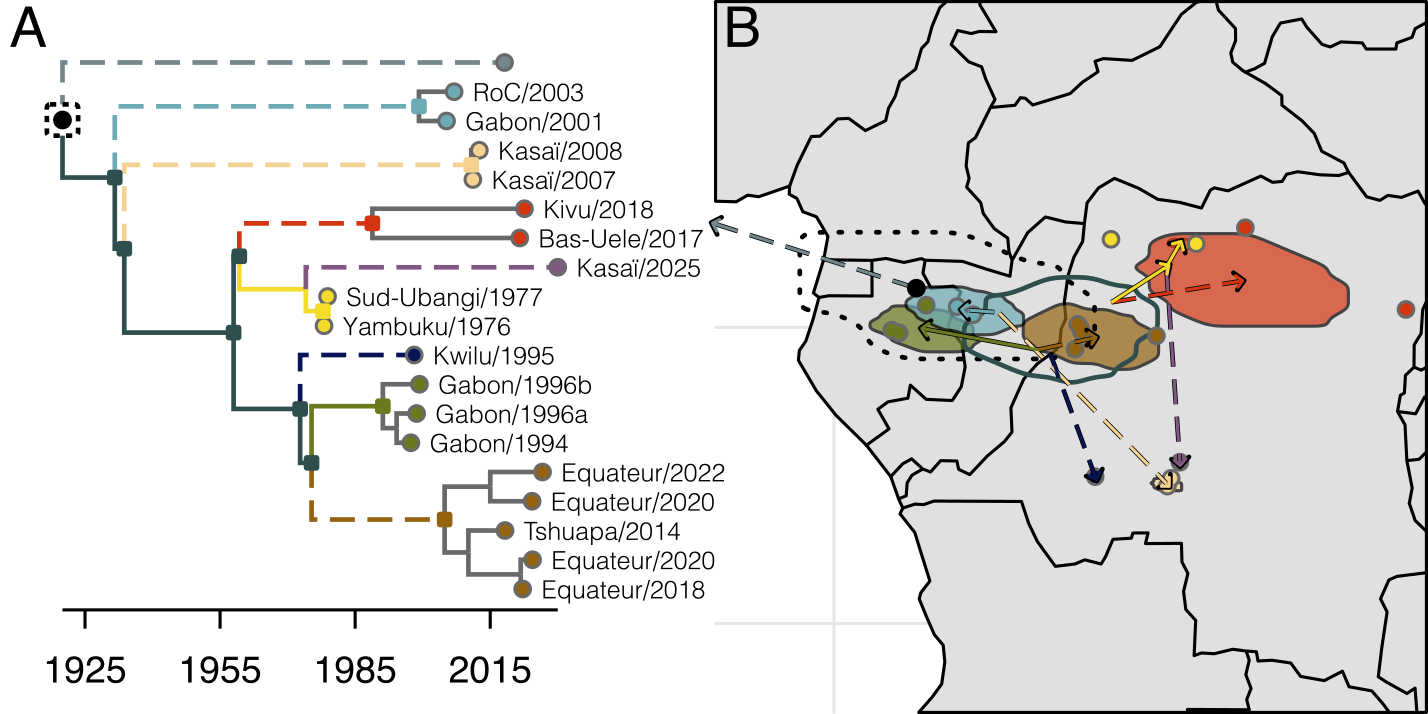
\includegraphics[width=1\textwidth]{figures/phyloGeo-full.png}
 \caption{\textbf{The geographic implication of latency in the EBOV reservoir including Makona/2013.} 
	Same as Figure~\ref{fig:scPhylogeo} but the Makona/2013 sample has been included in the analysis. 
   }
    \label{fig:scPhylogeoFull}
\end{figure*}

\begin{table}
    \centering
    \caption{\textbf{Recorded EBOV outbreaks used in this study.} Outbreak - the name of the outbreak; Country - the country of the outbreak; Adm1 - Administrative Region 1 of the outbreak. Duration - the dates of the outbreak. * indicates two genomes from the Equateur/2020 outbreak are present in our data.}
    
    \begin{tabular}{lllll}
Outbreak & Country  & Adm1  & Dates \\
\toprule
Yambuku/1976 & DRC & Mongala & Sep-Nov 1976 \\
Sud-Ubangi/1977 & DRC & Sud-Ubangi  & Jun-77 \\
Gabon/1994 & GAB & Ogooue-Ivindo & Dec 1994-Feb 1995 \\
Kwilu/1995 & DRC & Kwilu  & Jan-Jul 1995 \\
Gabon/1996a & GAB & Ogooue-Ivindo& Jan–Apr 1996 \\
Gabon/1996b & GAB & Ogooue-Ivindo  & Jul-96 \\
Gabon/2001 & GAB & Ogooue-Ivindo  & Oct 2001-Jul 2002 \\
% Mbomo-Kelle/2001 & COG & Cuvette Ouest & Lossi Animal Sanctuary & Dec 2001-May 2002 \\
% Mbomo-Kelle/2002 & COG & Cuvette Ouest & Kelle & Dec 2002–Apr 2003 \\
RoC/2003 & COG & Cuvette Ouest  & Oct-Dec 2003 \\
% Etoumbi/2005 & COG & Cuvette Ouest & Etoumbi & Apr-May 2005 \\
Kasaï/2007 & DRC & Kasai Occidental  & May-Nov 2007 \\
Kasaï/2008 & DRC & Kasai Occidental & Dec 2008–Feb 2009 \\
Makona/2013 & GIN & Gueckedou  & Dec 2013-Mar 2016 \\
Tshuapa/2014 & DRC & Tshuapa  & Aug–Nov 2014 \\
Bas-Uele/2017 & DRC & Bas Uele  & May-July 2017 \\
Equateur/2018 & DRC & Equateur & May-July 2018 \\
Kivu/2018 & DRC & Nord Kivu - Ituri - South Kiev & Aug 2018-June 2020 \\
Equateur/2020* & DRC & Equateur & June - Nov  2020 \\
Mbandaka/2022 & DRC & Equateur  & April- July 2022 \\
Kasaï/2025 & DRC & Kasai Occidental & August - October \\
\bottomrule
\end{tabular}
    \label{tab:oubtbreaks}
\end{table}

\begin{table}
\centering
\caption{\textbf{A list of the genomes used in this study with outbreak.} Accession refers to Pathoplexus accession and can be found at \cite{PP_SS_1057_2}. INSDC references the INSDC accesion for each sequence. Dataset denotes the smallest dataset in Table~\ref{tab:tipdater} which includes the taxa. Datasets build upon each other (e.g. the 11 taxa dataset adds 3 taxa to the 8 taxa dataset.)}

\begin{tabular}{llllll}
\toprule
Accession & INSDC & Country & Outbreak & Date & Dataset \\%& Authors\\
\toprule
PP\_000LS5R & KR063671 & DRC & Yambuku/1976 & 1976-10-01 & 8 taxa \\%&&\small{Das,S.R., Shabman,R., Halpin,R.A., Lin,X., Ransier,A., Fedorova,N., Tsitrin,T., Puri,V., Stockwell,T., Amedeo,P., Bishop,B., Gupta,N., Katzel,D., Schobel,S., Shrivastava,S., Alfson,K., Wentworth,D.E. and Griffiths,A.} \\
PP\_000LE61 & KC242791 & DRC & Sud-Ubangi/1977 & 1977-06 & 8 taxa \\%&&\small{Carroll,S.A., Towner,J.S., Sealy,T.K., McMullan,L.K., Khristova,M.L., Burt,F.J., Swanepoel,R., Rollin,P.E. and Nichol,S.T.}\\
PP\_000LE7Z & KC242792 & GAB & Gabon/1994 & 1994-12-27 & 8 taxa \\%&&\small{Carroll,S.A., Towner,J.S., Sealy,T.K., McMullan,L.K., Khristova,M.L., Burt,F.J., Swanepoel,R., Rollin,P.E. and Nichol,S.T.}\\
PP\_000MEGD & KU182905 & DRC & Kwilu/1995 & 1995-05-04 & 11 taxa \\%&&\small{Das,S.R., Shabman,R., Halpin,R.A., Akopov,A., Fedorova,N., Puri,V.,  Stockwell,T., Amedeo,P., Bishop,B., Katzel,D., Schobel,S., Shrivastava,S., Brasel,T., Yun,N., Paessler,S., Dowling,W. and Barrett,A. }\\
PP\_000LE8X & KC242793 & GAB & Gabon/1996a & 1996-02 & 8 taxa \\%&&\small{Carroll,S.A., Towner,J.S., Sealy,T.K., McMullan,L.K., Khristova,M.L., Burt,F.J., Swanepoel,R., Rollin,P.E. and Nichol,S.T. }\\
PP\_000LEGF & KC242798 & GAB & Gabon/1996b & 1996-10-27 & 8 taxa \\%&&\small{Carroll,S.A., Towner,J.S., Sealy,T.K., McMullan,L.K., Khristova,M.L., Burt,F.J., Swanepoel,R., Rollin,P.E. and Nichol,S.T. }\\
PP\_000LEJA & KC242800 & GAB & Gabon/2001 & 2002-02-23 & 8 taxa \\%&&\small{Carroll,S.A., Towner,J.S., Sealy,T.K., McMullan,L.K., Khristova,M.L., Burt,F.J., Swanepoel,R., Rollin,P.E. and Nichol,S.T. }\\
PP\_000LEQY & KF113529 & COG & RoC/2003 & 2003-10 & 8 taxa \\%&&\small{Chiu,C.Y., Naccache,S.N., Fair,J.N., Schneider,B.S. and Grard,G.} \\
PP\_000LDHD & HQ613403 & DRC & Kasaï/2007 & 2007-08-31 & 11 taxa \\%&&\small{ Grard,G., Biek,R., Muyembe-Tamfum,J.-J., Formenty,P., Paweska,J. and Leroy,E.} \\
PP\_000LDGG & HQ613402 & DRC & Kasaï/2008 & 2008-12-31 & 11 taxa \\%&&\small{ Grard,G., Biek,R., Muyembe-Tamfum,J.-J., Formenty,P., Paweska,J. and Leroy,E.}\\
PP\_000LETS & KJ660347 & GIN & Makona/2013 & 2014-03-20 & 8 taxa \\%&&\small{Baize,S., Pannetier,D., Oestereich,L., Rieger,T., Koivogui,L., Magassouba,N., Soropogui,B., Sow,M.S., Keita,S., De Clerck,H., Tiffany,A., Dominguez,G., Loua,M., Traore,A., Kolie,M., Malano,E.R., Heleze,E., Bocquin,A., Mely,S., Raoul,H., Caro,V., Cadar,D., Gabriel,M., Pahlmann,M., Tappe,D., Schmidt-Chanasit,J., Impouma,B., Diallo,A.K., Formenty,P., Van Herp,M. and Gunther,S.} \\
PP\_000LN4X & KP271018 & DRC & Tshuapa/2014 & 2014-08-20 & 19 taxa \\%&&\small{Naccache,S.N., Mbala,P., Ngay,I., Makuwa,M., Mulembakani,P., Muyembe,J.J., Schneider,B.S. and Chiu,C.Y.}\\
PP\_000NR4Q & MH613311 & DRC & Bas-Uele/2017 & 2017-05-07 & 19 taxa \\%&&\small{ Nsio,J., Kapetshi,J., Makiala,S., Formenty,P., Raymond,F., Tshapenda,G., Boucher,N., Corbeil,J., Okitandjate,A., Mbuyi,G., Kiyele,M., Mondonge,V., Kikoo,M.J., Van Herp,M., Rollin,P., Barboza,P., Muyembe Muzinga,B., Kalenga,O.I., Ahuka,S., Fausther-Bovendo,H., Kebela Ilunga,B., Kobinger,G.P. and Muyembe,J.-J.T. }\\
PP\_000NR9E & MH733477 & DRC & Equateur/2018 & 2018-05-10 & 19 taxa \\%&&\small{Mbala,P., Pratt,C., Wiley,M.R., Makiala-Mandanda,S., Aziza,A., Di Paola,N., Diagne,M.M., Chitty,J.A., Diop,M., Ayouba,A., Vidal,N., Faye,O., Karhemere,S., Aruna,A., Nsio,J., Mulangu,F., Mukadi,D., Mukadi,P., Kombe,J., Mulumba,A., Duraffour,S., Likofata,J., Pukuta,E., Minogue,T., Sozhamannan,S., Gross,S., Schroth,G., Delaporte,E., Sanchez-Lockhart,M., Peeters,M., Muyembe,J.-J., Alpha Sall,A., Palacios,G. and Ahuka-Mundeke,S. }\\
PP\_000NRSD & MK007330 & DRC & Kivu/2018 & 2018-07-28 & 19 taxa \\%&&\small{ Mbala-Kingebeni,P., Aziza,A., Di Paola,N., Wiley,M.R., Makiala-Mandanda,S., Caviness,K., Pratt,C.B., Prieto,K., Chitty,J.A., Larson,P., Ayouba,A., Vidal,N., Karhemere,S., Diop,M., Diagne,M.M., Faye,M., Faye,O., Aruna,A., Nsio,J., Mulanga,F., Mukadi,D., Mukadi,P., Kombe,J., Mulumba,A., Duraffour,S., Likofata,J., Pukuta,E., Gonzalez,J., Bartlett,M.L., Sozhamannan,S., Gross,S., Schroth,G., Kuhn,J., Delaporte,E., Sanchez-Lockhart,M., Alpha Sall,A., Muyembe,J.-J., Peeters,M., Palacios,G. and Ahuka-Mundeke,S. }\\
PP\_000PJZ4 & OR084849 & DRC & Equateur/2020 & 2020-05-31 & 19 taxa \\%&&\small{ Kinganda-Lusamaki,E., Whitmer,S., Lokilo-Lofiko,E., Amuri-Aziza,A., Muyembe-Mawete,F., Makangara-Cigolo,J.C., Makaya,G., Mbuyi,F., Whitesell,A., Kallay,R., Choi,M., Pratt,C., Mukadi-Bamuleka,D., Kavunga-Membo,H., Matondo-Kuamfumu,M., Mambu-Mbika,F., Ekila-Ifinji,R., Shoemaker,T., Stewart,M., Eng,J., Rajan,A., Soke,G.N., Fonjungo,P.N., Otshudiema,J.O., Folefack,G.L.T., Pukuta-Simbu,E., Talundzic,E., Shedroff,E., Bokete,J.L., Legand,A., Formenty,P., Mores,C.N., Porzucek,A.J., Tritsch,S.R., Kombe,J., Tshapenda,G., Mulangu,F., Ayouba,A., Delaporte,E., Peeters,M., Wiley,M.R., Montgomery,J.M., Klena,J.D., Muyembe-Tamfum,J.-J., Ahuka-Mundeke,S. and Mbala-Kingebeni,P.}\\
PP\_000PJVC & OR084846 & DRC & Equateur/2020 & 2020-06-12 & 19 taxa \\%&&\small{Kinganda-Lusamaki,E., Whitmer,S., Lokilo-Lofiko,E., Amuri-Aziza,A., Muyembe-Mawete,F., Makangara-Cigolo,J.C., Makaya,G., Mbuyi,F., Whitesell,A., Kallay,R., Choi,M., Pratt,C., Mukadi-Bamuleka,D., Kavunga-Membo,H., Matondo-Kuamfumu,M., Mambu-Mbika,F., Ekila-Ifinji,R., Shoemaker,T., Stewart,M., Eng,J., Rajan,A., Soke,G.N., Fonjungo,P.N., Otshudiema,J.O., Folefack,G.L.T., Pukuta-Simbu,E., Talundzic,E., Shedroff,E., Bokete,J.L., Legand,A., Formenty,P., Mores,C.N., Porzucek,A.J., Tritsch,S.R., Kombe,J., Tshapenda,G., Mulangu,F., Ayouba,A., Delaporte,E., Peeters,M., Wiley,M.R., Montgomery,J.M., Klena,J.D., Muyembe-Tamfum,J.-J., Ahuka-Mundeke,S. and Mbala-Kingebeni,P. }\\
PP\_003V5NQ & - & DRC & Equateur/2022 & 2022-04-25 & 19 taxa \\%& &\small{Placide Mbala-Kingebeni, Jean-Jacques Muyembe, Steve Ahuka-Mundeke, Hugo Kavunga, Daniel Mukadi, Elisabeth Pukuta, Eddy Kinganda Lusamaki, Amuri Aziza, Jean Claude Makangara, Emmanuel Lokilo, Franck Edidi, Junior Bula Bula, Raphael Lumembe, Gabriel Kabamba, Fabrice Mambu, Joel Montgomery, Peter Fonjungo, Norbert Soke, Jacques Likofata, Vital Mondonge, Gervais Folefack, Prosper Djiguimde, John Otshudiema, Deby Mukendi, Dieudonné Mwamba, John Kombe, Sofonias Tessema, Didi Bofaka, Andrew Rambaut, Mike Wiley, Catherine Pratt}\\
PP\_003RXHG & - & DRC & Kasaï/2025 & 2025-09-01 & 19 taxa \\%&&\small{Adrienne Amuri-Aziza, Gradi Luakanda - Ndelemo, Jean-Claude Makangara-Cigolo, Prince Akil-Bandali, Princesse Paku-Tshambu, Sam Wilkinson, Louis Tshulo, Josh Quick, Andre Citenga, Chloe Muswamba-Kayembe, Olga Ntumba-Tshitenge, Emmanuel Lokilo-Lofiko, Fiston Cikaya-Kankolongo, Ola Rilia, Servet Kimbonza, Elisabeth Pukuta, Daniel Mukadi, Christian Ngandu, Mathias Mossoko, Gabriel Kabamba -Lungenyi, Raphael Lumembe-Numbi, Elzedeck Mabika-Bope, Patrick Mukadi, Catherine Pratt, Dieudonne Mwamba, Nick Loman, Andrew Rambaut, Eddy Kinganda-Lusamaki, Tony Wawina-Bokalanga, Dieudonne Mumba - Ngoyi, Jean-Jacques Muyembe-Tamfum, Steve Ahuka-Mundeke  Placide Mbala-Kingebeni }\\
\bottomrule
\end{tabular}
\label{tab:genomes}
\end{table}


\pagebreak

\section*{Supplemental text}



\subsubsection*{Further exploration of temporal signal}

The temporal outliers observed in the EBOV phylogeny could have resulted from enhanced purifying selection instead of latency.
To investigate this possibility, we repeated the analysis in Figure~\ref{fig:rtt} with a partition made of only third position codon sites and intergenic regions (Figure~\ref{fig:rtt-cds3_ig}).
Despite elevated evolutionary rates, which are expected for a dataset enriched in synonymous sites, this analysis produced the same conclusions as that run on the full genome.
Temporal outliers were maintained, as were our initial observations regarding within- and between-cluster rates. 

\begin{figure*}[!hbtp]
    \centering
    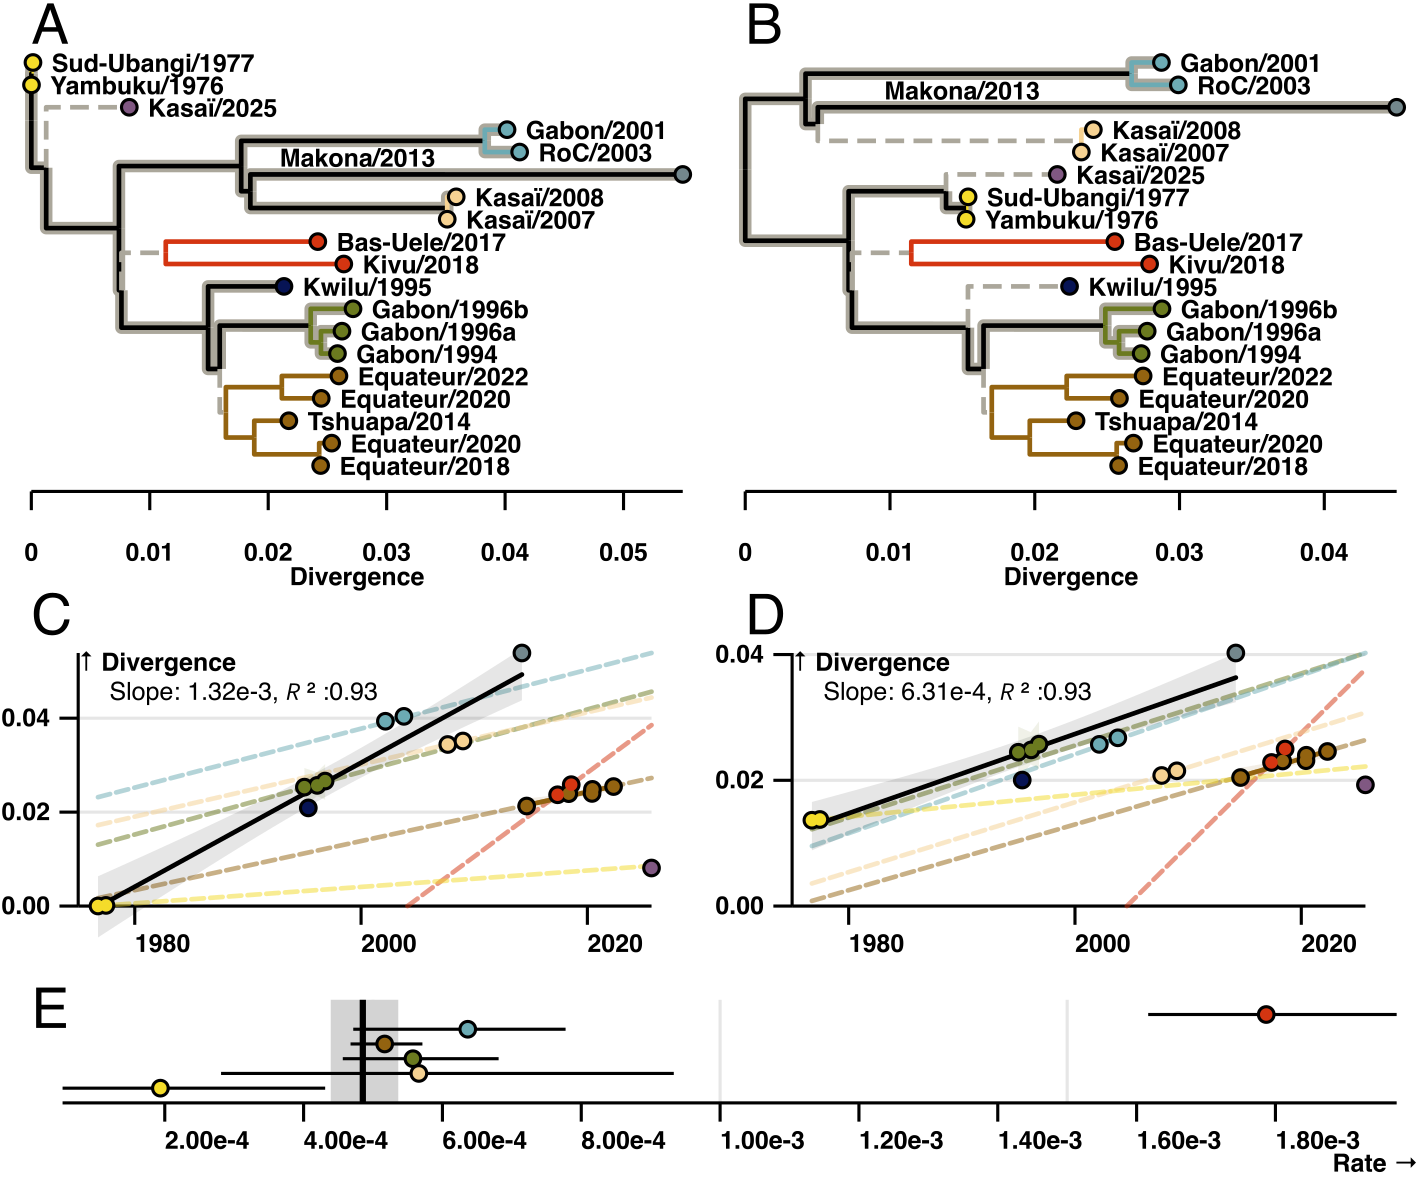
\includegraphics[width=0.8\textwidth]{figures/rtt-cds3_ig.png} 
     \caption{\textbf{Rate heterogeneity in the EBOV phylogeny (third position coding sites and intergenic regions).}
	Same as Figure~\ref{fig:rtt} with the exception that the presented phylogenies were made with only sites in the third codon position and intergenic regions.
	}    \label{fig:rtt-cds3_ig}
\end{figure*}


\subsection*{Prior sensitivity analysis}

Preliminary analyses suggested that when applied to the EBOV dataset the latency model is positioned between two extremes, both of which likely have identifiability issues.
If the rate of latent-replicating transition is too low relative to the scale of the tree, no latency is expected and the model reduces to a strict-clock model.
In this case, there is no temporal signal in the full dataset if a strick-clock model is employed.
The evolutionary rate is unidentifiable.

If the rate of transition is too high then the model approaches a free-rates model with an evolutionary rate on each branch. 
In some datasets where the parameters of the latency model may be known this could be tolerated.
However, our analyses show that we have little power to predict \emph{a priori} the amount of latency on a latent branch.
Note the wide spread in the distribution of time spent latent in Figure~\ref{fig:future}B. 

In this study we place a gamma prior on the rate of latent-replicating transitions.
The gamma distribution was parameterized with a rate parameter equal to the root height.
This prior was chosen to ensure the expected rate of latency scales with the phylogeny and strikes a balance between the extremes above without prohibiting either.
As noted in the methods, this prior favors no latency while still allowing for the possibility of latency (95\% prior probability of no latency).

We ran two additional analyses to explore the impact of this prior on our findings.
In the first, the rate of the gamma distribution was set to one half the root height, which would favor more latency (Figure~\ref{fig:nM-rh05}).
In the other, the rate of the gamma distribution was set to twice the root height, which favors less latency (Figure~\ref{fig:nM-rh2}).
Both analyses produced comparable results to that presented in the main text (Table \ref{tab:prior} and Figures~\ref{fig:nM-rh2} \& \ref{fig:nM-rh05}).
In fact, increasing the rate of the gamma prior by a factor of two increased the posterior support for the proposed root to nearly 90\% (Figures~\ref{fig:nM-rh2}).

\begin{table}[!hbp]
    \centering
    
\begin{tabular}{lrrr}
    Prior & Root age & Clock rate & Latent branches  \\ 
\toprule
Root height & 1929 [1887,1957]& 2.34$ \times 10^{-4}$ [1.41, 3.19] & 6 [5,9] \\
Root height $\div 2$ & 1924 [1878,1957] & 2.34$ \times 10^{-4}$ [1.42, 3.21] & 7 [5,11]\\
Root height $\times 2$ & 1934 [1903,1958] & 2.29$ \times 10^{-4}$ [1.36,3.08] & 6 [4,8] \\
\bottomrule
\end{tabular}
  \caption{\textbf{Prior sensitivity analysis.} Prior - the rate parameter of the gamma distribution placed on the latent rate. Root age- posterior mean and 95\% HPD of the root age. Clock rate- posterior mean and 95\% HPD of the evolutionary rate when replicating. Latent branches -  the median and 95\% HPD of the number of branches with at least one latent period.}
    \label{tab:prior}
\end{table}

\begin{figure*}[!hbtp]
    \centering
    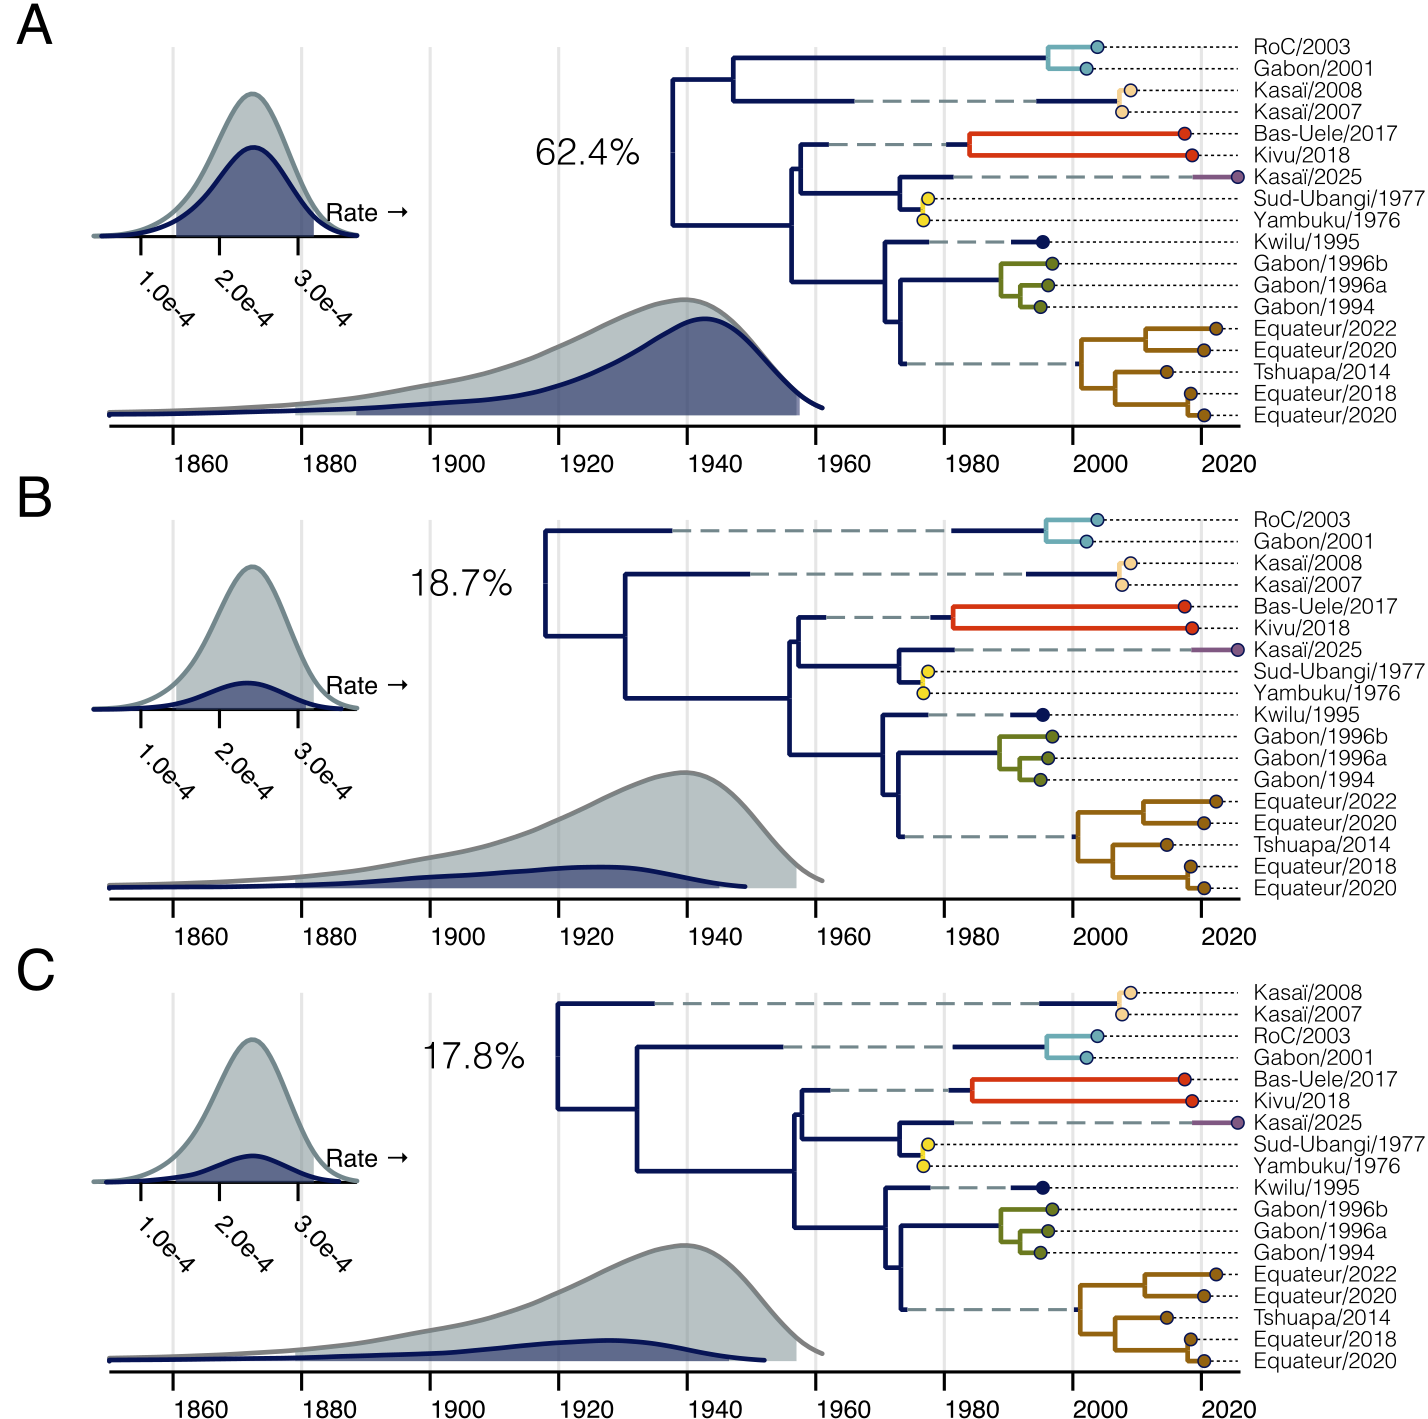
\includegraphics[width=1\textwidth]{figures/allRoots.noMakona-rh0.5.png}
  \caption{\textbf{Evolutionary history of EBOV in Central Africa with a prior favoring more latency.}
	Same as Figure~\ref{fig:nMallRoots}; however the rate parameter of gamma prior placed on the rate of latent transitions is one-half the root height.
    }
    \label{fig:nM-rh05}
\end{figure*}

\begin{figure*}[!hbtp]
    \centering
    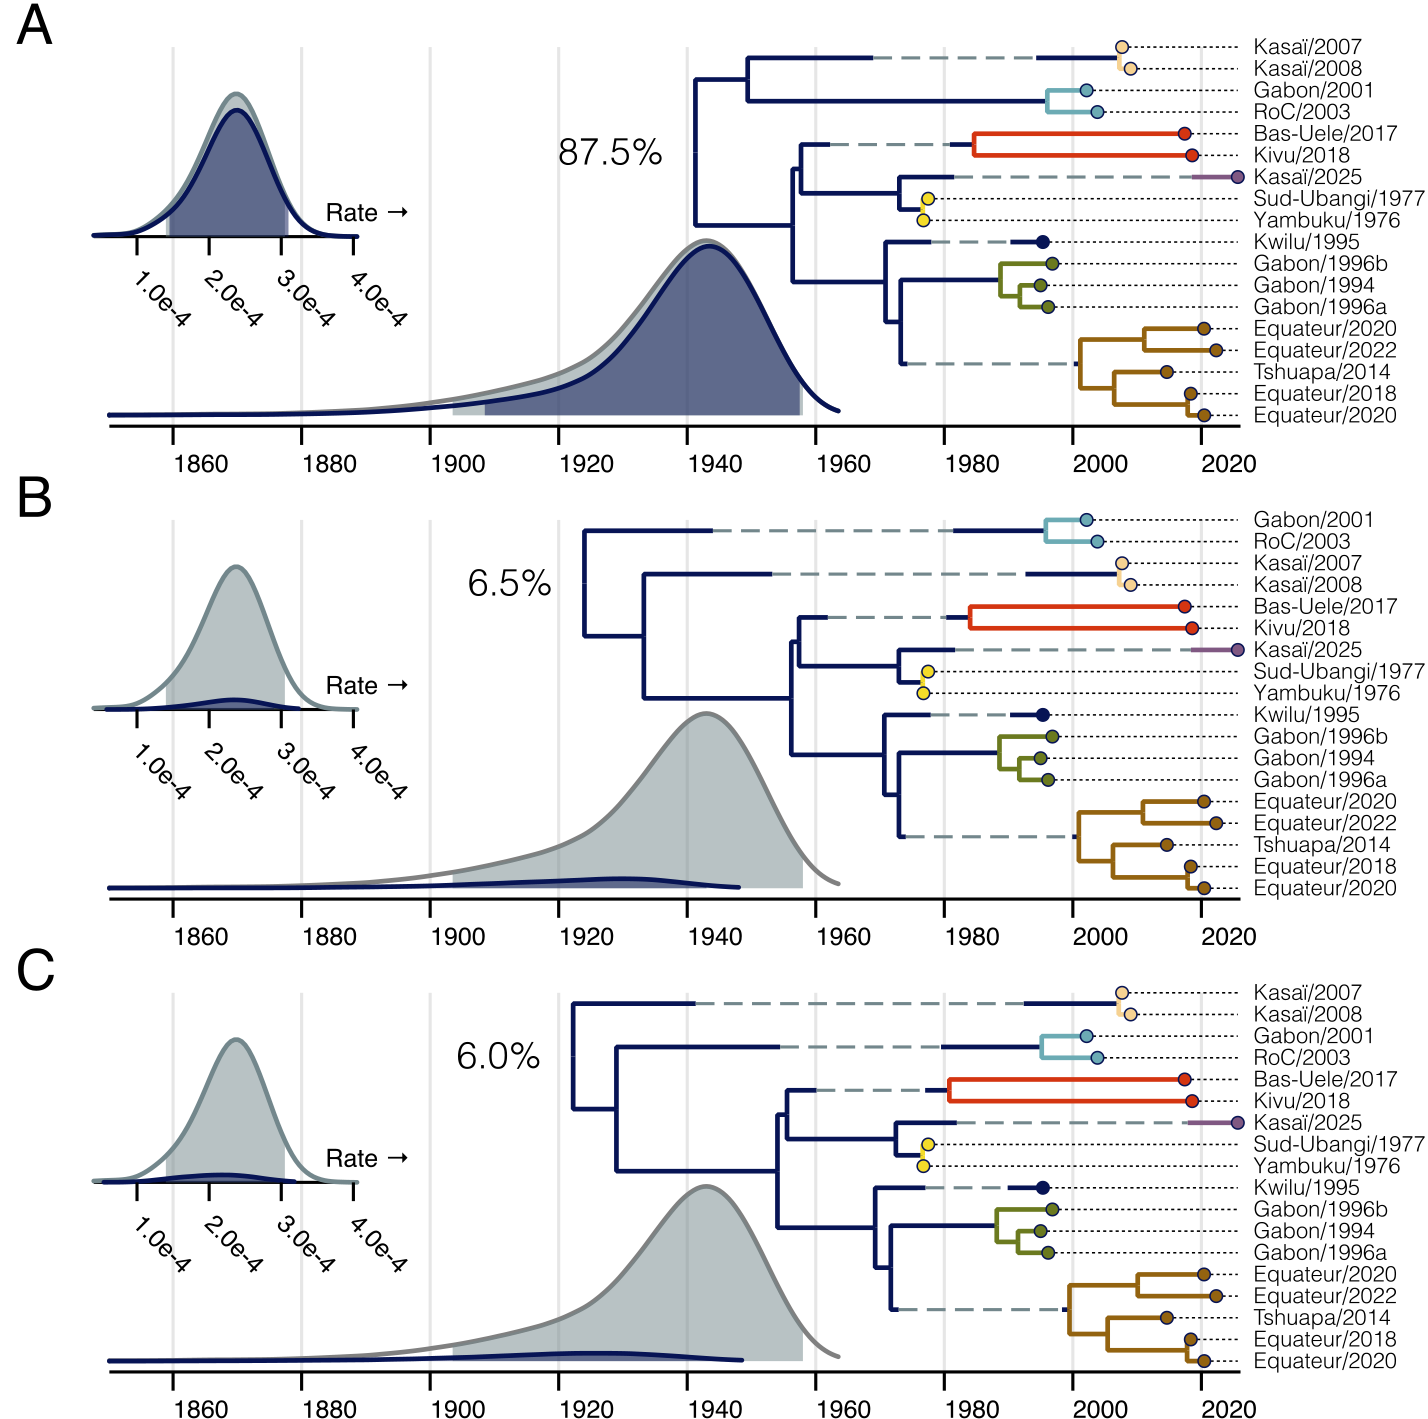
\includegraphics[width=1\textwidth]{figures/allRoots.noMakona-rh2.png}
    \caption{\textbf{Evolutionary history of EBOV in Central Africa with a prior favoring less latency.}
	Same as Figure~\ref{fig:nMallRoots}; however the rate parameter of gamma prior place the rate of latent transitions is twice the root height.
    }
    \label{fig:nM-rh2}
\end{figure*}

